
\subsection{Two Dimensional Plot Types}
\PGFPlots\ supports several two-dimensional line-plots like piecewise linear line plots, piecewise constant plots, smoothed plots, bar plots and comb plots. Most of them use the \PGF\ plot handler library directly, see \cite[section 18.8]{tikz}.

Plot types are part of the plot style, so they are set with options. Most of the basic 2d plot types are part of \Tikz, see \cite[section 18.8]{tikz}, and are probably known to users of \Tikz. They are documented here as well.


\subsubsection{Linear Plots}
\begin{plottype}{sharp plot}
Linear (`sharp') plots are the default. Point coordinates are simply connected by straight lines. 
\begin{codeexample}[]
\begin{tikzpicture}
\begin{axis}
	\addplot+[sharp plot] coordinates 
		{(0,0) (1,2) (2,3)};
\end{axis}
\end{tikzpicture}
\end{codeexample}

The `|+|' here means to use the normal plot cycle list and append `|sharp plot|' to its option list.
\end{plottype}

\subsubsection{Smooth Plots}
\begin{plottype}{smooth}
Smooth plots interpolate smoothly between successive points.
\begin{codeexample}[]
\begin{tikzpicture}
\begin{axis}
	\addplot+[smooth] coordinates 
		{(0,0) (1,2) (2,3)};
\end{axis}
\end{tikzpicture}
\end{codeexample}
\end{plottype}

\subsubsection{Constant Plots}
Constant plots draw lines parallel to the $x$-axis to connect coordinates. The discontinuous edges may be drawn or not, and marks may be placed on left or right ends.

\begin{plottype}{const plot}
Connects all points with horizontal and vertical lines. Marks are placed left-handed on horizontal line segments, causing the plot to be right-sided continuous at all data points.

\begin{codeexample}[]
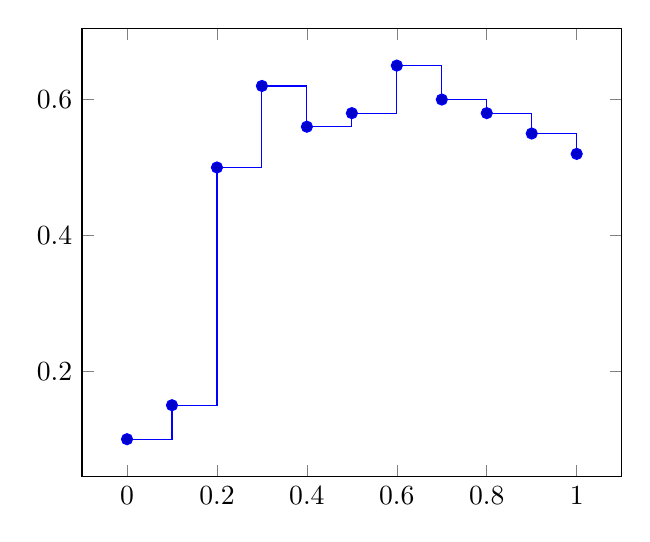
\begin{tikzpicture}
\begin{axis}
\addplot+[const plot]
coordinates
{(0,0.1)    (0.1,0.15)  (0.2,0.5)   (0.3,0.62)
 (0.4,0.56) (0.5,0.58)  (0.6,0.65)  (0.7,0.6)
 (0.8,0.58) (0.9,0.55)  (1,0.52)};
\end{axis}
\end{tikzpicture}
\end{codeexample}


\begin{codeexample}[]
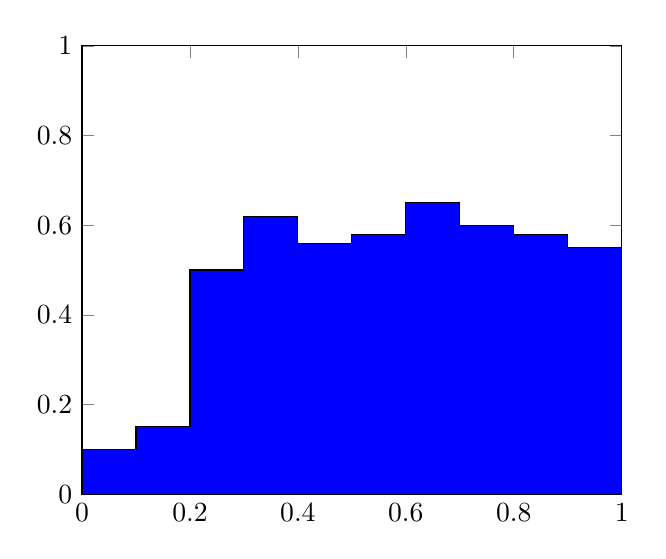
\begin{tikzpicture}
\begin{axis}[ymin=0,ymax=1,enlargelimits=false]
\addplot
	[const plot,fill=blue,draw=black] 
coordinates
{(0,0.1)    (0.1,0.15)  (0.2,0.5)   (0.3,0.62)
 (0.4,0.56) (0.5,0.58)  (0.6,0.65)  (0.7,0.6)
 (0.8,0.58) (0.9,0.55)  (1,0.52)} 
	\closedcycle;
\end{axis}
\end{tikzpicture}
\end{codeexample}
\end{plottype}

\begin{plottype}{const plot mark left}
An alias for `|const plot|'.
\end{plottype}

\begin{plottype}{const plot mark right}
 A variant which places marks on the right of each line segment, causing plots to be left-sided continuous at coordinates.
\begin{codeexample}[]
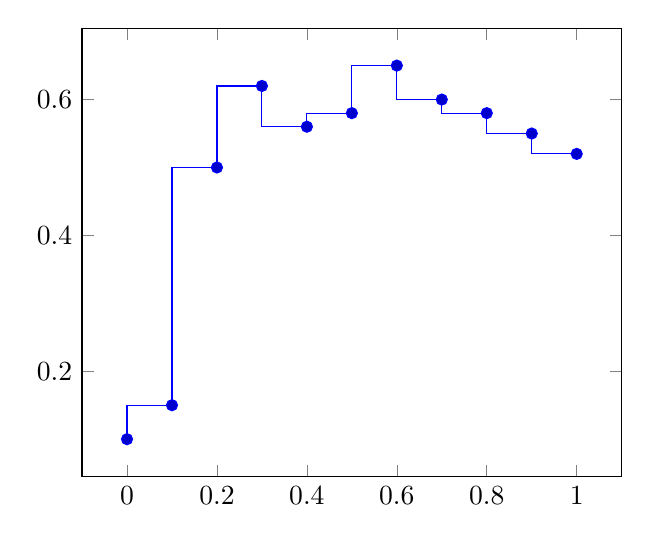
\begin{tikzpicture}
\begin{axis}
\addplot+[const plot mark right]
coordinates
{(0,0.1)    (0.1,0.15)  (0.2,0.5)   (0.3,0.62)
 (0.4,0.56) (0.5,0.58)  (0.6,0.65)  (0.7,0.6)
 (0.8,0.58) (0.9,0.55)  (1,0.52)};
\end{axis}
\end{tikzpicture}
\end{codeexample}
\end{plottype}

\begin{plottype}{jump mark left}
A variant of `|const plot mark left|' which does not draw vertical lines.
\begin{codeexample}[]
\begin{tikzpicture}
\begin{axis}[samples=8]
\addplot+[jump mark left,domain=-5:0] 
	{4*x^2 - 5};

\addplot+[jump mark right,domain=-5:0] 
	{0.7*x^3 + 50};
\end{axis}
\end{tikzpicture}
\end{codeexample}
\end{plottype}

\begin{plottype}{jump mark right}
A variant of `|const plot mark right|' which does not draw vertical lines.
\end{plottype}

\subsubsection{Bar Plots}
Bar plots place horizontal or vertical bars at coordinates. Multiple bar plots in one axis can be stacked on top of each other or aligned next to each other.

\begin{plottype}{xbar}
	Places horizontal bars between the $(y=0)$ line and each coordinate.

	This option is used on a per-plot basis and configures only the visualization of coordinates. The figure-wide style |/pgfplots/xbar| also sets reasonable options for ticks, legends and multiple plots.
\begin{codeexample}[]
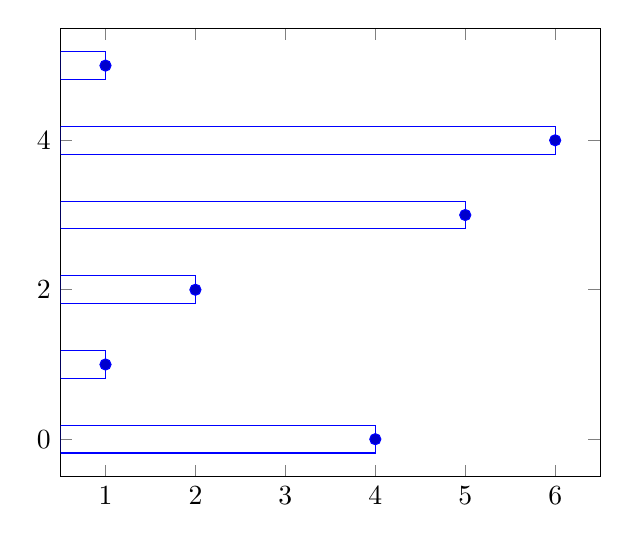
\begin{tikzpicture}
\begin{axis}
\addplot+[xbar] coordinates 
	{(4,0) (1,1) (2,2) 
	 (5,3) (6,4) (1,5)};
\end{axis}
\end{tikzpicture}
\end{codeexample}
	Bars are centered at plot coordinates with width |bar width|. Using bar plots usually means more than just a different way of how to connect coordinates, for example to draw ticks outside of the axis, change the legend's appearance or introduce shifts if multiple |\addplot| commands appear.

	There is a preconfigured style for |xbar| which is installed automatically if you provide |xbar| as argument to the axis environment which provides this functionality.
% \usetikzlibrary{patterns}
\begin{codeexample}[]
\begin{tikzpicture}
\begin{axis}[xbar,enlargelimits=0.15]
\addplot
[draw=blue,pattern=horizontal lines light blue] 
coordinates
	{(10,5) (15,10) (5,15) (24,20) (30,25)};

\addplot
[draw=black,pattern=horizontal lines dark blue] 
coordinates 
	{(3,5) (5,10) (15,15) (20,20) (35,25)};
\end{axis}
\end{tikzpicture}
\end{codeexample}
Here |xbar| yields |/pgfplots/xbar| because it is an argument to the axis, not to a single plot.

	Besides line-, fill- and colorstyles, bars can be configured with |bar width| and |bar shift|, see below.
\end{plottype}

\begin{stylekey}{/pgfplots/xbar=\marg{shift for multiple plots} (default 2pt)}
	This style sets |/tikz/xbar| \emph{and} some commonly used options concerning horizontal bars for the complete axis. This is automatically done if you provide |xbar| as argument to an axis argument, see above.

The |xbar| style defines shifts if multiple plots are placed into one axis. It draws bars adjacent to each other, separated by \marg{shift for multiple plots}. Furthermore, it sets the style |bar cycle list| and sets tick and legend appearance options.

The style is defined as follows.
\begin{codeexample}[code only]
\pgfplotsset{
	/pgfplots/xbar/.style={
		/tikz/xbar,
		bar cycle list,
		tick align=outside,
		xbar legend,
		/pgf/bar shift={%
			% total width = n*w + (n-1)*skip
			% i.e. subtract half for centering
			-0.5*(\numplotsofactualtype*\pgfplotbarwidth + (\numplotsofactualtype-1)*#1)  + 
			% the '0.5*w' is for centering
			(.5+\plotnumofactualtype)*\pgfplotbarwidth + \plotnumofactualtype*#1%
		},
	},
}
\end{codeexample}
The formular for |bar shift| assigns shifts dependent on the total number of plots and the current plot's number. It is designed to fill a total width of $n \cdot $|bar width|$ + (n-1) \cdot $\marg{shift for multiple plots}. The $0.5$ compensates for centering.
\end{stylekey}

\begin{plottype}{ybar}
	Like |xbar|, this option generates bar plots. It draws vertical bars between the ($x=0$) line and each input coordinate.
\begin{codeexample}[]
\begin{tikzpicture}
\begin{axis}
\addplot+[ybar] plot coordinates
	{(0,3) (1,2) (2,4) (3,1) (4,2)};
\end{axis}
\end{tikzpicture}
\end{codeexample}
	The example above simply changes how input coordinates shall be visualized. As mentioned for |xbar|, one usually needs modified legends and shifts for multiple bars in the same axis.

	There is a predefined style which installs these customizations when provided to the axis-environment:
\begin{codeexample}[]
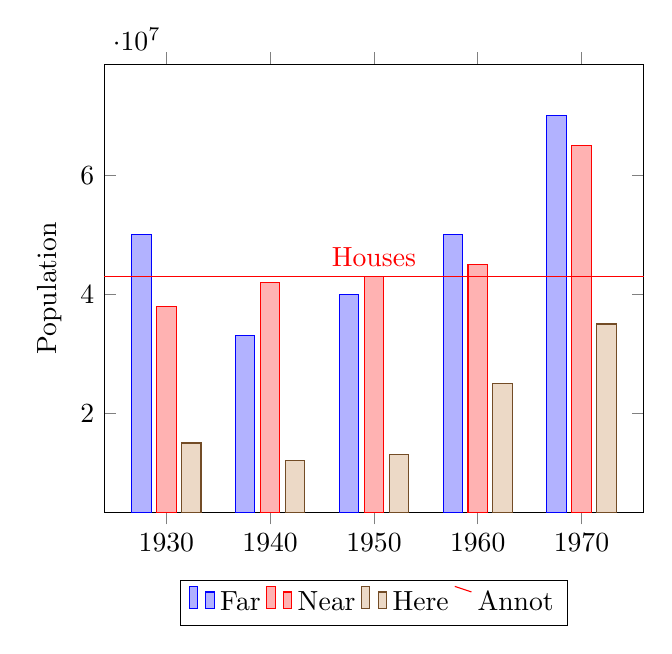
\begin{tikzpicture}
\begin{axis}[
	x tick label style={
		/pgf/number format/1000 sep=},
	ylabel=Population,
	enlargelimits=0.15,
	legend style={at={(0.5,-0.15)},
		anchor=north,legend columns=-1},
	ybar,
	bar width=7pt,
]
\addplot 
	coordinates {(1930,50e6) (1940,33e6)
		 (1950,40e6) (1960,50e6) (1970,70e6)};

\addplot 
	coordinates {(1930,38e6) (1940,42e6) 
		(1950,43e6) (1960,45e6) (1970,65e6)};

\addplot 
	coordinates {(1930,15e6) (1940,12e6) 
		(1950,13e6) (1960,25e6) (1970,35e6)};

\addplot[red,sharp plot,update limits=false] 
	coordinates {(1910,4.3e7) (1990,4.3e7)} 
	node[above] at (axis cs:1950,4.3e7) {Houses};

\legend{Far,Near,Here,Annot}
\end{axis}
\end{tikzpicture}
\end{codeexample}
Here |ybar| yields |/pgfplots/ybar| because it is an argument to the axis, not to a single plot. The style affects the first three |\addplot| commands. Note that it shifts them horizontally around the plot coordinates. The fourth |\addplot| command is some kind of annotation which doesn't |update limits|.

	As for |xbar|, the bar width and shift can be configured with |bar width| and |bar shift|. However, the bar shift is better provided as argument to |/pgfplots/ybar| since this style will overwrite the bar shift. Thus, prefer |/pgfplots/ybar=4pt| to set the bar shift.

	Sometimes it is useful to write the $y$ values directly near the bars. This can be realized using the |nodes near coords| method:
\begin{codeexample}[]
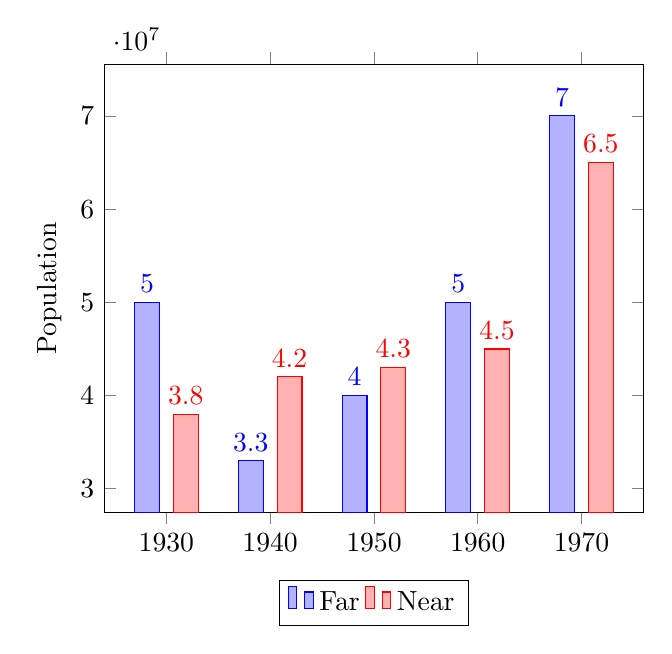
\begin{tikzpicture}
\begin{axis}[
	x tick label style={
		/pgf/number format/1000 sep=},
	ylabel=Population,
	enlargelimits=0.15,
	legend style={at={(0.5,-0.15)},
		anchor=north,legend columns=-1},
	ybar=5pt,% configures `bar shift'
	bar width=9pt,
	nodes near coords,
	point meta=y *10^-7 % the displayed number
]
\addplot 
	coordinates {(1930,50e6) (1940,33e6)
		 (1950,40e6) (1960,50e6) (1970,70e6)};

\addplot 
	coordinates {(1930,38e6) (1940,42e6) 
		(1950,43e6) (1960,45e6) (1970,65e6)};

\legend{Far,Near}
\end{axis}
\end{tikzpicture}
\end{codeexample}
\end{plottype}

\begin{stylekey}{/pgfplots/ybar=\marg{shift for multiple plots} (default 2pt)}
	As |/pgfplots/xbar|, this style sets the |/tikz/ybar| option to draw vertical bars, but it also provides commonly used options for vertical bars.

	If you supply |ybar| to an axis environment, |/pgfplots/ybar| will be chosen instead of |/tikz/ybar|.

	It changes the legend, draws ticks outside of the axis lines and draws multiple |\addplot| arguments adjacent to each other; block--centered at the $x$ coordinate and separated by \marg{shift for multiple plots}. It will also install the |bar shift| for |every node near coord|. Furthermore, it installs the style |bar cycle list|. It is defined similarly to |/pgfplots/xbar|.
\end{stylekey}

\begin{pgfplotskey}{bar cycle list}
	A style which installs cycle lists for multiple bar plots.
\begin{codeexample}[code only]
\pgfplotsset{
	/pgfplots/bar cycle list/.style={/pgfplots/cycle list={%
		{blue,fill=blue!30!white,mark=none},%
		{red,fill=red!30!white,mark=none},%
		{brown!60!black,fill=brown!30!white,mark=none},%
		{black,fill=gray,mark=none},%
		}
	},
}
\end{codeexample}
	
\end{pgfplotskey}

\begin{key}{/pgf/bar width=\marg{dimension} (initially 10pt)}
	Configures the width used by |xbar| and |ybar|. It is accepted to provide mathematical expressions.
\end{key}

\begin{key}{/pgf/bar shift=\marg{dimension} (initially 0pt)}
	Configures a shift for |xbar| and |ybar|. Use |bar shift| together with |bar width| to draw multiple bar plots into the same axis. It is accepted to provide mathematical expressions.
\end{key}


\begin{plottype}{ybar interval}
	This plot type produces vertical bars with width (and shift) relatively to intervals of coordinates.

	There is one conceptional difference when working with intervals: an interval is defined by \emph{two} coordinates. Since |ybar| has one value for each interval, the $i$th bar is defined by
	\begin{enumerate}
		\item the $y$ value of the $i$th coordinates,
		\item the $x$ value of the $i$th coordinate as left interval boundary,
		\item the $x$ value of the $(i+1)$th coordinate as right interval boundary.
	\end{enumerate}
	Consequently, there is \emph{one coordinate too much}: the last coordinate will \emph{only} be used to determine the interval width; its $y$ value doesn't influence the bar appearance.

	It is installed on a per-plot basis and configures \emph{only} the visualization of coordinates. See the style |/pgfplots/ybar interval| which configures the appearance of the complete figure.
\begin{codeexample}[]
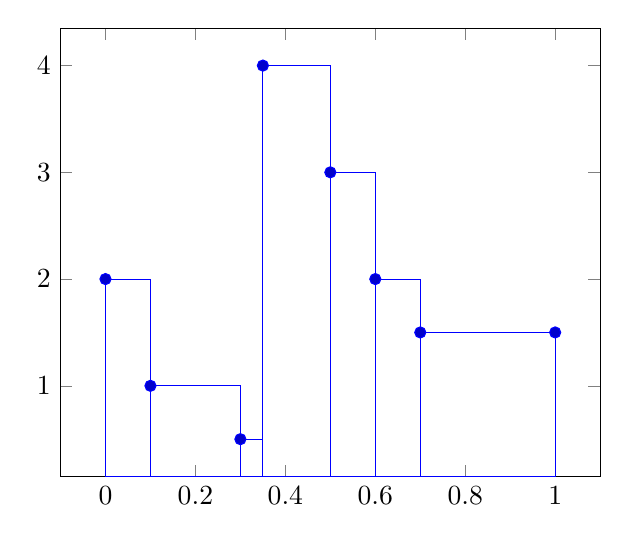
\begin{tikzpicture}
\begin{axis}
\addplot+[ybar interval] plot coordinates
	{(0,2) (0.1,1) (0.3,0.5) (0.35,4) (0.5,3)
	 (0.6,2) (0.7,1.5) (1,1.5)};
\end{axis}
\end{tikzpicture}
\end{codeexample}

\begin{codeexample}[]
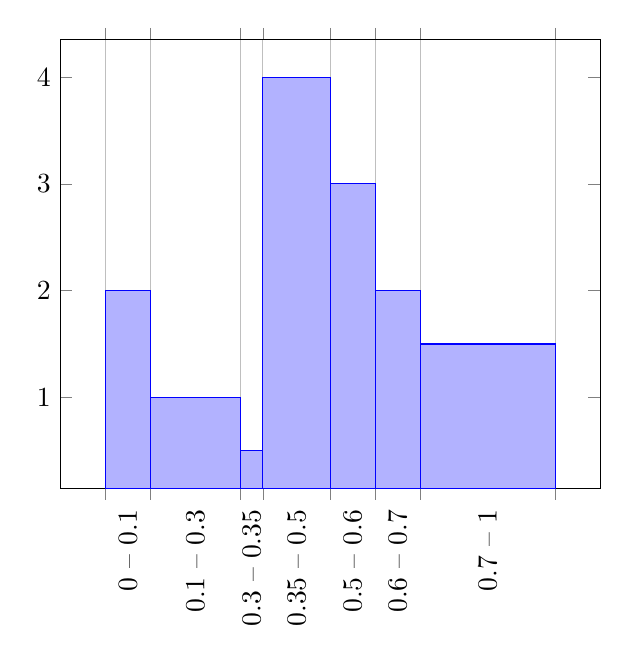
\begin{tikzpicture}
\begin{axis}[ybar interval,
	xtick=data,
	xticklabel interval boundaries,
	x tick label style=
		{rotate=90,anchor=east}
	]
\addplot coordinates
	{(0,2) (0.1,1) (0.3,0.5) (0.35,4) (0.5,3)
	 (0.6,2) (0.7,1.5) (1,1.5)};
\end{axis}
\end{tikzpicture}
\end{codeexample}

\begin{codeexample}[]
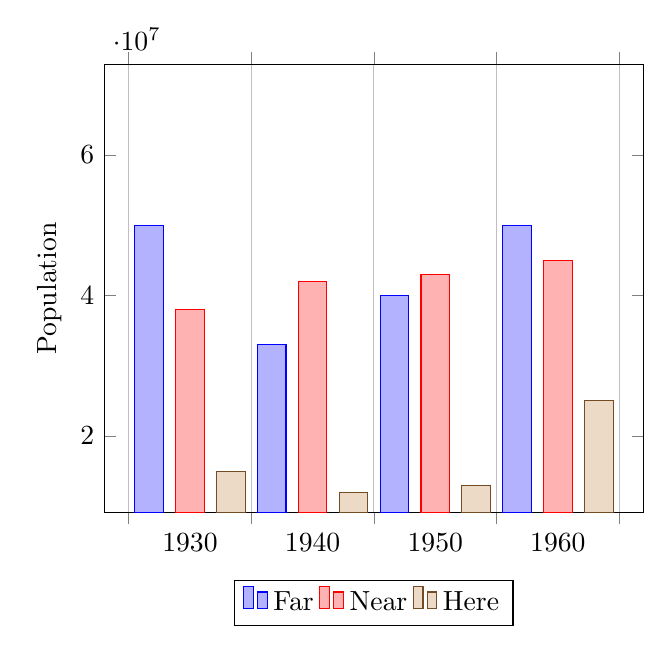
\begin{tikzpicture}
\begin{axis}[
	x tick label style={
		/pgf/number format/1000 sep=},
	ylabel=Population,
	enlargelimits=0.05,
	legend style={at={(0.5,-0.15)},
		anchor=north,legend columns=-1},
	ybar interval=0.7,
]
\addplot 
	coordinates {(1930,50e6) (1940,33e6)
		 (1950,40e6) (1960,50e6) (1970,70e6)};

\addplot 
	coordinates {(1930,38e6) (1940,42e6) 
		(1950,43e6) (1960,45e6) (1970,65e6)};

\addplot 
	coordinates {(1930,15e6) (1940,12e6) 
		(1950,13e6) (1960,25e6) (1970,35e6)};
\legend{Far,Near,Here}
\end{axis}
\end{tikzpicture}
\end{codeexample}
\end{plottype}

\begin{stylekey}{/pgfplots/ybar interval=\marg{relative width} (default 1)}
	A style which is intended to install options for |ybar interval| for a complete figure. This includes tick and legend appearance, management of multiple bar plots in one figure and a more adequate |cycle list| using the style |bar cycle list|.
\end{stylekey}

\begin{plottype}{xbar interval}
	As |ybar interval|, just for horizontal bars. 
\begin{codeexample}[]
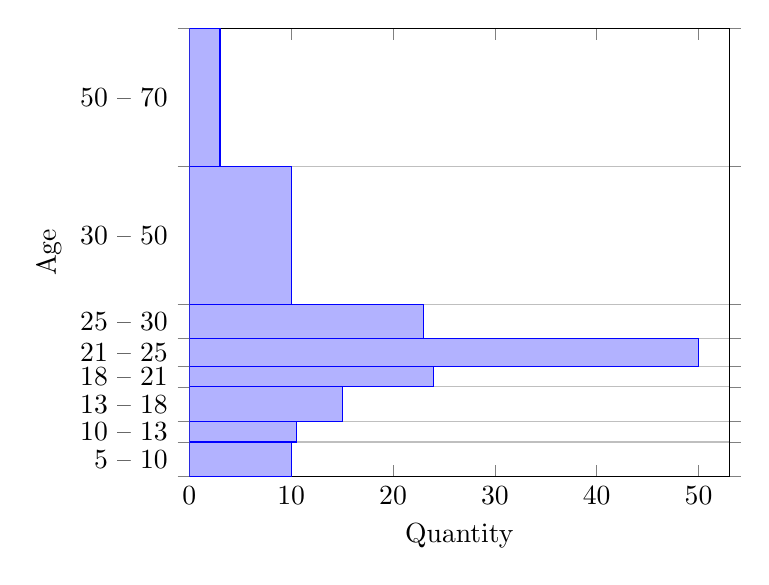
\begin{tikzpicture}
\begin{axis}[
	xmin=0,xmax=53,
	ylabel=Age,
	xlabel=Quantity,
	enlargelimits=false,
	ytick=data,
	yticklabel interval boundaries,
	xbar interval,
]
\addplot
	coordinates {(10,5) (10.5,10) (15,13) 
		(24,18) (50,21) (23,25) (10,30) 
		(3,50) (3,70)};
\end{axis}
\end{tikzpicture}
\end{codeexample}
\end{plottype}

\begin{stylekey}{/pgfplots/xbar interval=\marg{relative width} (default 1)}
	A style which is intended to install options for |xbar interval| for a complete figure, see the style |/pgfplots/ybar interval| for details.
\end{stylekey}

\begin{pgfplotsxykey}{\x ticklabel interval boundaries}
	These are style keys which set |x tick label as interval| (see page~\pageref{key:pgfplots:ticklabelasinterval} for details) and configure the tick appearance to be \marg{start} -- \marg{end} for each tick interval.
\end{pgfplotsxykey}

\subsubsection{Comb Plots}
Comb plots are very similar to bar plots except that they employ single horizontal/vertical lines instead of rectangles.

\begin{plottype}{xcomb}
\begin{codeexample}[]
\begin{tikzpicture}
\begin{axis}
\addplot+[xcomb] coordinates 
	{(4,0) (1,1) (2,2) 
	 (5,3) (6,4) (1,5)};
\end{axis}
\end{tikzpicture}
\end{codeexample}
\end{plottype}

\begin{plottype}{ycomb}
\begin{codeexample}[]
\begin{tikzpicture}
\begin{axis}
\addplot+[ycomb] plot coordinates
	{(0,3) (1,2) (2,4) (3,1) (4,2)};
\end{axis}
\end{tikzpicture}
\end{codeexample}
\end{plottype}

\subsubsection{Stacked Plots}
\begin{pgfplotskey}{stack plots=\mchoice{x,y,false} (initially false)}
	Allows stacking of plots in either $x$ or $y$ direction. Stacking means to add either $x$- or $y$ coordinates of successive |\addplot| commands on top of each other.
\begin{codeexample}[]
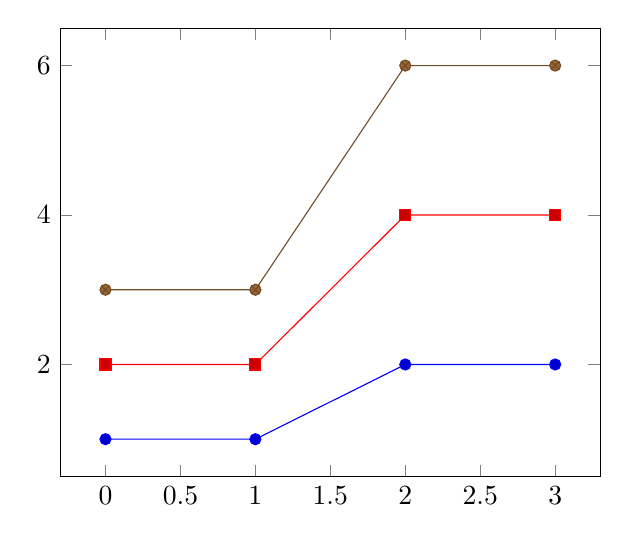
\begin{tikzpicture}
	\begin{axis}[stack plots=y]
	\addplot coordinates
		{(0,1) (1,1) (2,2) (3,2)};
	\addplot coordinates
		{(0,1) (1,1) (2,2) (3,2)};
	\addplot coordinates
		{(0,1) (1,1) (2,2) (3,2)};
	\end{axis}
\end{tikzpicture}
\end{codeexample}

|stack plots| is particularly useful for bar plots. The following examples demonstrate its functionality. Normally, it is advisable to use the styles |ybar stacked| and |xbar stacked| which also set some other options.
\begin{codeexample}[]
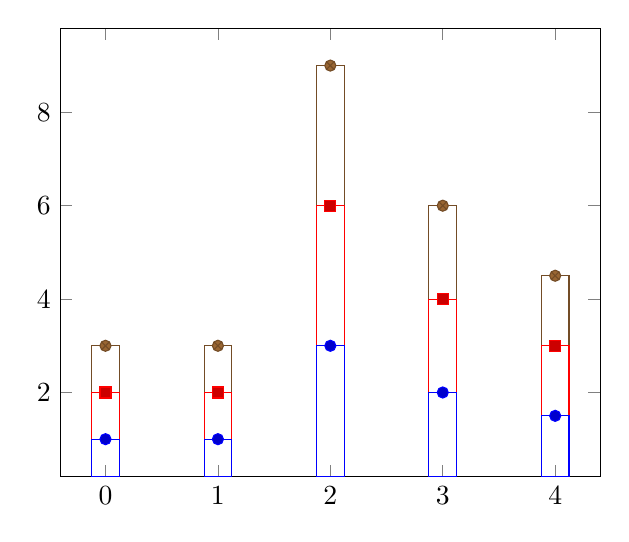
\begin{tikzpicture}
	\begin{axis}[stack plots=y,/tikz/ybar]
	\addplot coordinates
		{(0,1) (1,1) (2,3) (3,2) (4,1.5)};
	\addplot coordinates
		{(0,1) (1,1) (2,3) (3,2) (4,1.5)};
	\addplot coordinates
		{(0,1) (1,1) (2,3) (3,2) (4,1.5)};
	\end{axis}
\end{tikzpicture}
\end{codeexample}

\begin{codeexample}[]
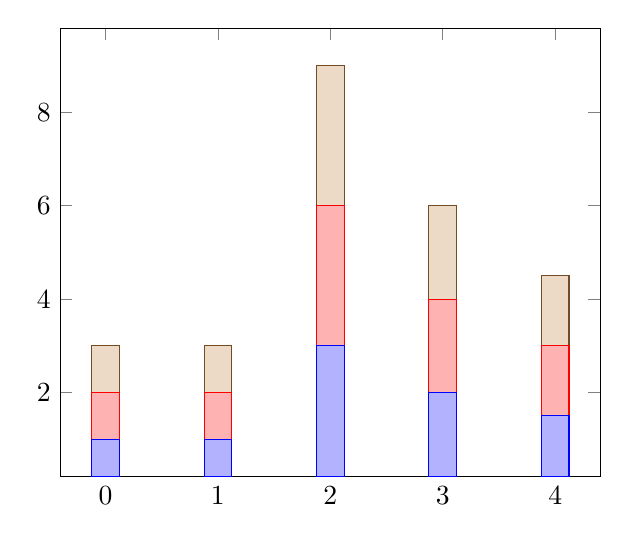
\begin{tikzpicture}
	\begin{axis}[ybar stacked]
	\addplot coordinates
		{(0,1) (1,1) (2,3) (3,2) (4,1.5)};
	\addplot coordinates
		{(0,1) (1,1) (2,3) (3,2) (4,1.5)};
	\addplot coordinates
		{(0,1) (1,1) (2,3) (3,2) (4,1.5)};
	\end{axis}
\end{tikzpicture}
\end{codeexample}

\begin{codeexample}[]
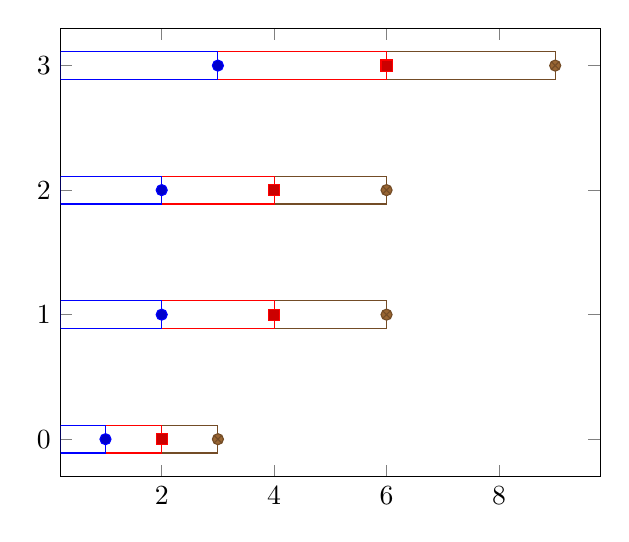
\begin{tikzpicture}
	\begin{axis}[stack plots=x,/tikz/xbar]
	\addplot coordinates
		{(1,0) (2,1) (2,2) (3,3)};
	\addplot coordinates
		{(1,0) (2,1) (2,2) (3,3)};
	\addplot coordinates
		{(1,0) (2,1) (2,2) (3,3)};
	\end{axis}
\end{tikzpicture}
\end{codeexample}
\begin{codeexample}[]

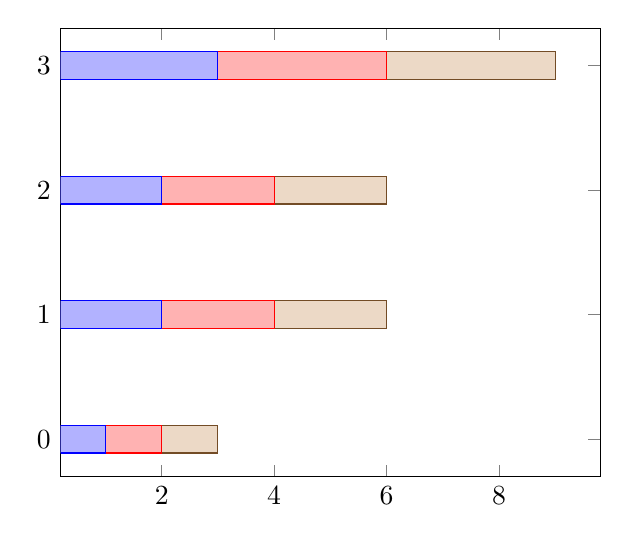
\begin{tikzpicture}
	\begin{axis}[xbar stacked]
	\addplot coordinates
		{(1,0) (2,1) (2,2) (3,3)};
	\addplot coordinates
		{(1,0) (2,1) (2,2) (3,3)};
	\addplot coordinates
		{(1,0) (2,1) (2,2) (3,3)};
	\end{axis}
\end{tikzpicture}
\end{codeexample}
The current implementation for |stack plots| does \emph{not} interpolate missing coordinates. That means stacking will fail if the plots have different grids.
\end{pgfplotskey}

\begin{pgfplotskey}{stack dir=\mchoice{plus,minus} (initially plus)}
	Configures the direction of |stack plots|. The value |plus| will add coordinates of successive plots while |minus| subtracts them.
\end{pgfplotskey}

\begin{pgfplotskey}{reverse stacked plots=\mchoice{true,false} (initially true, default true)}
	Configures the sequence in which stacked plots are drawn. This is more or less a technical detail which should not be changed in any normal case.

	The motivation is as follows: suppose multiple |\addplot| commands are stacked on top of each other and they are processed in the order of appearance. Than, the second plot could easily draw its lines (or fill area) on top of the first one - hiding its marker or line completely. Therefor, \PGFPlots\ reverses the sequence of drawing commands.

	This has the side-effect that any normal \Tikz-paths inside of an axis will also be processed in reverse sequence.
\end{pgfplotskey}

\begin{stylekey}{/pgfplots/xbar stacked=\mchoice{plus,minus} (default plus)}
	A figure-wide style which enables stacked horizontal bars (i.e.\ |xbar| and |stack plots=x|). It also adjusts the legend and tick appearance and assigns a useful |cycle list|.
\end{stylekey}
\begin{stylekey}{/pgfplots/ybar stacked=\mchoice{plus,minus} (default plus)}
	A figure-wide style which enables stacked vertical bars (i.e.\ |ybar| and |stack plots=y|). It also adjusts the legend and tick appearance and assigns a useful |cycle list|.
\end{stylekey}

\begin{stylekey}{/pgfplots/xbar interval stacked=\mchoice{plus,minus} (default plus)}
	A style similar to |/pgfplots/xbar stacked| for the interval based bar plot variant.
\end{stylekey}
\begin{stylekey}{/pgfplots/ybar interval stacked=\mchoice{plus,minus} (default plus)}
	A style similar to |/pgfplots/ybar stacked| for the interval based bar plot variant.
\end{stylekey}

\subsubsection{Area Plots}
Area plots are a combination of |\closedcycle| and |stack plots|. They can be combined with any other plot type.

\begin{codeexample}[]
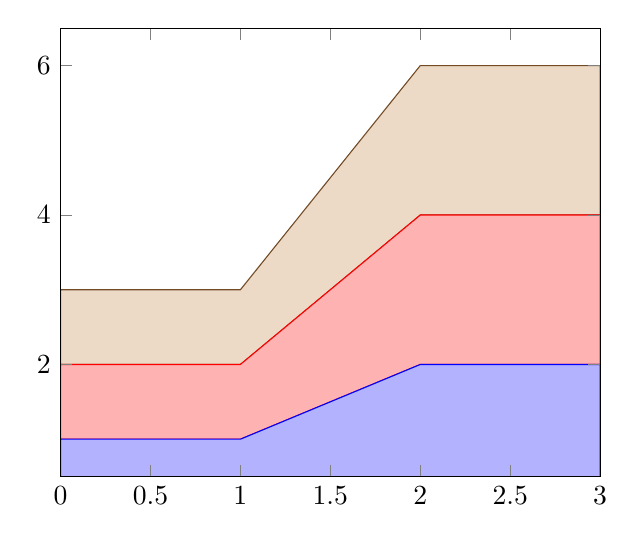
\begin{tikzpicture}
	\begin{axis}[
		stack plots=y,
		area style,
		enlarge x limits=false]
	\addplot coordinates
		{(0,1) (1,1) (2,2) (3,2)} 
		\closedcycle;
	\addplot coordinates
		{(0,1) (1,1) (2,2) (3,2)}
		\closedcycle;
	\addplot coordinates
		{(0,1) (1,1) (2,2) (3,2)}
		\closedcycle;
	\end{axis}
\end{tikzpicture}
\end{codeexample}
\noindent
Area plots may need modified legends, for example using the |area legend| key. Furthermore, one may want to consider the |axis on top| key such that filled areas do not overlap ticks and grid lines. 

\begin{stylekey}{/pgfplots/area style}
	A style which sets
\begin{codeexample}[code only]
\pgfplotsset{
	/pgfplots/area style/.style={%
		area cycle list,
		area legend,
		axis on top,
	}}
\end{codeexample}
\end{stylekey}

\begin{stylekey}{/pgfplots/area cycle list}
	A style which installs a |cycle list| suitable for area plots. The initial configuration of this style simply invokes the |bar cycle list| which does also provide filled plot styles.
\end{stylekey}

\begin{codeexample}[]
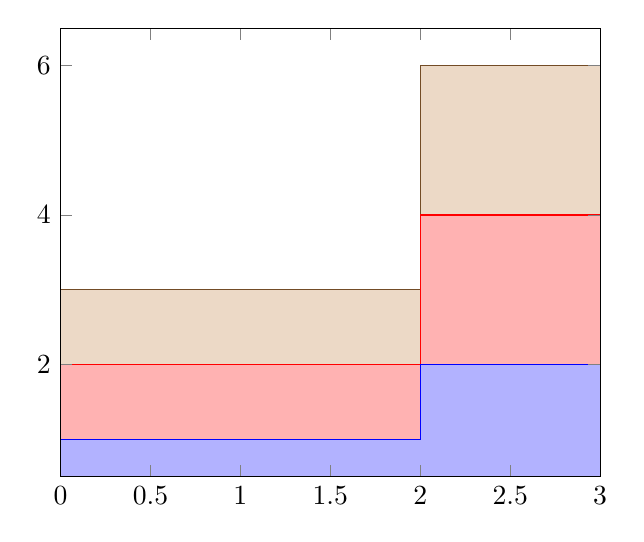
\begin{tikzpicture}
	\begin{axis}[
		const plot,
		stack plots=y,
		area style,
		enlarge x limits=false]
	\addplot coordinates
		{(0,1) (1,1) (2,2) (3,2)} 
		\closedcycle;
	\addplot coordinates
		{(0,1) (1,1) (2,2) (3,2)}
		\closedcycle;
	\addplot coordinates
		{(0,1) (1,1) (2,2) (3,2)}
		\closedcycle;
	\end{axis}
\end{tikzpicture}
\end{codeexample}

\begin{codeexample}[]
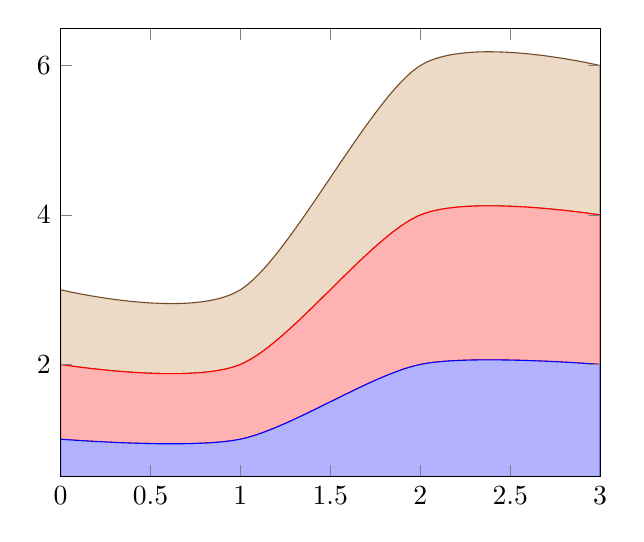
\begin{tikzpicture}
	\begin{axis}[
		smooth,
		stack plots=y,
		area style,
		enlarge x limits=false]
	\addplot coordinates
		{(0,1) (1,1) (2,2) (3,2)} 
		\closedcycle;
	\addplot coordinates
		{(0,1) (1,1) (2,2) (3,2)}
		\closedcycle;
	\addplot coordinates
		{(0,1) (1,1) (2,2) (3,2)}
		\closedcycle;
	\end{axis}
\end{tikzpicture}
\end{codeexample}

\begin{codeexample}[]
\pgfplotstableread{pgfplots.timeseries.dat}\loadedtable
\pgfplotstabletypeset\loadedtable
\end{codeexample}
\begin{codeexample}[]
\pgfplotstableread
	{pgfplots.timeseries.dat}
	{\loadedtable}

\begin{tikzpicture}
	\begin{axis}[
		ymin=0,
		minor tick num=4,
		enlarge x limits=false,
		axis on top,
		every axis plot post/.append style=
			{mark=none},
		const plot,
		legend style={
			area legend,
			at={(0.5,-0.15)},
			anchor=north,
			legend columns=-1}]

	\addplot[draw=blue,fill=blue!30!white]
	 table[x=time,y=1minload] from \loadedtable
		\closedcycle;
	\addplot table[x=time,y=nodes] from \loadedtable;
	\addplot table[x=time,y=cpus] from \loadedtable;
	\addplot table[x=time,y=processes] 
		from \loadedtable;
	\legend{1min load,nodes,cpus,processes}
	\end{axis}
\end{tikzpicture}
\end{codeexample}

\begin{codeexample}[width=4cm]
\pgfplotstableread{pgfplots.timeseries.dat}\loadedtable

\begin{tikzpicture}
	\begin{axis}[
		ymin=0,
		minor tick num=4,
		enlarge x limits=false,
		const plot,
		axis on top,
		stack plots=y,
		cycle list={%
			{blue!70!black,fill=blue},%
			{blue!60!white,fill=blue!30!white},%
			{draw=none,fill={rgb:red,138;green,82;blue,232}},%
			{red,thick}%
		},
		ylabel={Mem [GB]},
		legend style={
			area legend,
			at={(0.5,-0.15)},
			anchor=north,
			legend columns=2}]

	\addplot table[x=time,y=memused]      from \loadedtable \closedcycle;
	\addplot table[x=time,y=memcached]    from \loadedtable \closedcycle;
	\addplot table[x=time,y=membuf]       from \loadedtable \closedcycle;
	\addplot+[stack plots=false]
			 table[x=time,y=memtotal]     from \loadedtable;
	\legend{Memory used,Memory cached,Memory buffered,Total memory}
	\end{axis}
\end{tikzpicture}
\end{codeexample}

\subsubsection{Scatter Plots}
\label{sec:pgfplots:scatter:2d}
The most simple scatter plots produce the same as the line plots above -- but they contain only markers. They are enabled using the |only marks| key of \Tikz.
\begin{plottype}{only marks}
Draws a simple scatter plot: all markers have the same appearance.
\begin{codeexample}[]
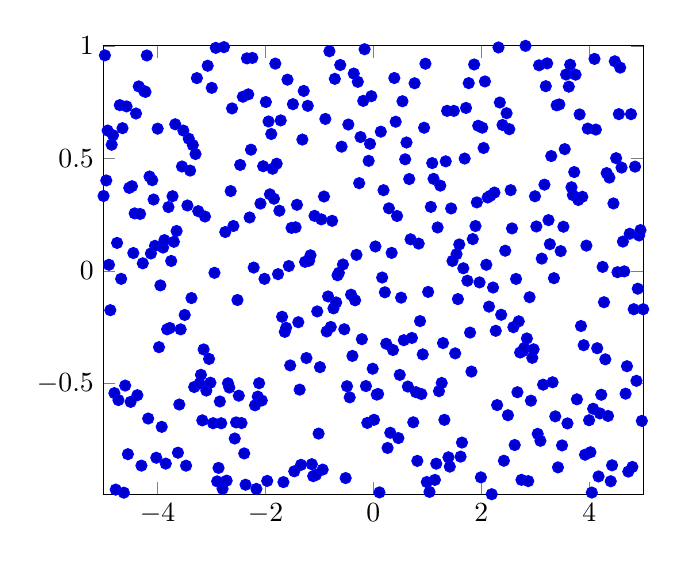
\begin{tikzpicture}
	\begin{axis}[enlargelimits=false]
	\addplot+[only marks,samples=400]
		{rand};
	\end{axis}
\end{tikzpicture}
\end{codeexample}
	The |only marks| visualization style simply draws marks at every coordinate. Marks can be set with |mark=|\meta{mark name} and marker options like size and color can be specified using the |mark options=|\marg{style options} key (or by modifying the |every mark| style). The available markers along with the accepted style options can be found in section~\ref{sec:markers} on page~\pageref{sec:markers}.
\end{plottype}

\label{pgfplots:scatter}
More sophisticated scatter plots change the marker appearance for each data point. An example is that marker colors depend on the magnitude of function values $f(x)$ or other provided coordinates. The term ``scatter plot'' will be used for this type of plots in the following sections.

Scatter plots require ``source'' coordinates. These source coordinates can be the $y$ coordinate, or explicitly provided additional values.

\begin{plottype}[/pgfplots]{scatter}
	Enables marker appearance modifications. The default implementation acquires ``source coordinates'' for every data point (see |scatter src| below) and maps them linearly into the current color map. The resulting color is used as draw and fill color of the marker.

\begin{codeexample}[]
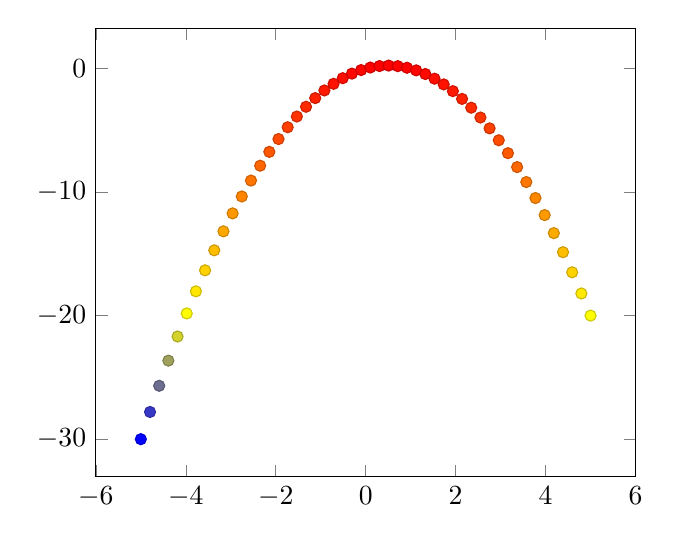
\begin{tikzpicture}
	\begin{axis}
	\addplot+[scatter,only marks,
		 samples=50,scatter src=y]
		{x-x^2};
	\end{axis}
\end{tikzpicture}
\end{codeexample}

	The key |scatter| is simply a boolean variable which enables marker modifications. It applies only to markers and it can be combined with any other plot type.

\begin{codeexample}[]
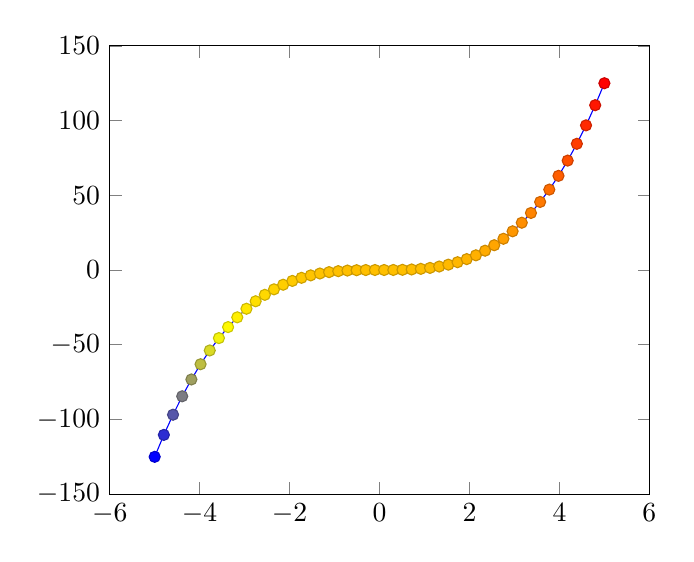
\begin{tikzpicture}
	\begin{axis}
	\addplot+[scatter,
		 samples=50,scatter src=y]
		{x^3};
	\end{axis}
\end{tikzpicture}
\end{codeexample}
\end{plottype}

Scatter plots can be configured using a set of options. One of them is mandatory, the rest allows fine grained control over marker appearance options.

\begin{pgfplotskey}{scatter src=\mchoice{none,\meta{expression},x,y,z,f(x),explicit,explicit symbolic} (initially none)}
\label{pgfplots:scatter:src}
	This key is necessary for any scatter plot and it is set to |f(x)| as soon as |scatter| is activated and no different choice has been made. It needs to be provided as \marg{option} for |\addplot| to configure the value used to determine marker appearances. Actually, |scatter src| is nothing but an alias for |point meta|, so the main documentation for this key is on page~\pageref{pgfplots:pointmeta}. However, we summarize the choices here together with scatter plot examples.

	Usually, |scatter src| provides input data (numeric or string type) which is used to determine colors and other style options for markers.
	The default configuration expects numerical data which is mapped linearly into the current color map.

	The value of |scatter src| determines how to get this data: the choices \declaretext{x}, \declaretext{y} and \declaretext{z} will use either the $x$, $y$ or $z$ coordinates to determine marker options. Any coordinate filters, logarithms or stacked-plot computations have already been applied to these values (use |rawx|, |rawy| and |rawz| for unprocessed values). The special choice |f(x)| is the same as |y| for two dimensional plots and the same as |z| for three dimensional plots. The choice \declaretext{explicit} expects the scatter source data as additional coordinate from the coordinate input streams (see section~\ref{pgfplots:providing:input} for how to provide input meta data or below for some small examples). They will be treated as numerical data. The choice \declaretext{explicit symbolic} also expects scatter source data as additional meta information for each input coordinate, but it treats them as strings,  not as numerical data. Consequently, no arithmetics is performed. It is task of the scatter plot style to do something with it. See, for example, the |scatter/classes| style below.
	Finally, it is possible to provide an arbitrary mathematical expression which involves zero, one or more of the values \declaretext{x} (the current $x$ coordinate), \declaretext{y} (the current $y$ coordinate) or \declaretext{z} (the current $z$ coordinate, if any).

	If data is read from tables, mathematical expressions might also involve |\thisrow|\marg{column name} or |\thisrowno|\marg{column index} to access any of the table cells in the current row.

	Here are examples for how to provide data for the choices \declaretext{explicit} and \declaretext{explicit symbolic}.
\begin{codeexample}[code only]
\begin{tikzpicture}
	\begin{axis}
		% provide color data explicitly using [<data>]
		% behind coordinates:
		\addplot+[scatter,scatter src=explicit]
			coordinates {
				(0,0) [1.0e10]
				(1,2) [1.1e10]
				(2,3) [1.2e10]
				(3,4) [1.3e10]
				% ...
			};

        % Assumes a datafile.dat like
        % xcolname  ycolname    colordata
        % 0         0           0.001
        % 1         2           0.3
        % 2         2.1         0.4
        % 3         3           0.5
        % ...
        % the file may have more columns.
		\addplot+[scatter,scatter src=explicit]
			table[x=xcolname,y=ycolname,meta=colordata] 
				{datafile.dat};
		% Same data as last example: 
		\addplot+[scatter,scatter src=\thisrow{colordata}+\thisrow{ycolname}]
			table[x=xcolname,y=ycolname] 
				{datafile.dat};

        % Assumes a datafile.dat like
        % 0         0           0.001
        % 1         2           0.3
        % 2         2.1         0.4
        % 3         3           0.5
        % ...
        % the first three columns will be used here:
		\addplot+[scatter,scatter src=explicit]
			file {datafile.dat};
	\end{axis}
\end{tikzpicture}
\end{codeexample}

	Please note that |scatter src|$\neq$|none| results in computational work even if |scatter=false|.
\end{pgfplotskey}

\begin{stylekey}{/pgfplots/scatter/use mapped color=\marg{options for each marker} (initially draw=mapped color!80!black,fill=mapped color)}
	This style is installed by default. When active, it recomputes the color |mapped color| for every processed point coordinate by transforming the |scatter src| coordinates into the current color map linearly. Then, it evaluates the options provided as \marg{options for each marker} which are expected to depend on |mapped color|.

	The user interface for color maps is described in section~\ref{pgfplots:colormap}.
\begin{codeexample}[]
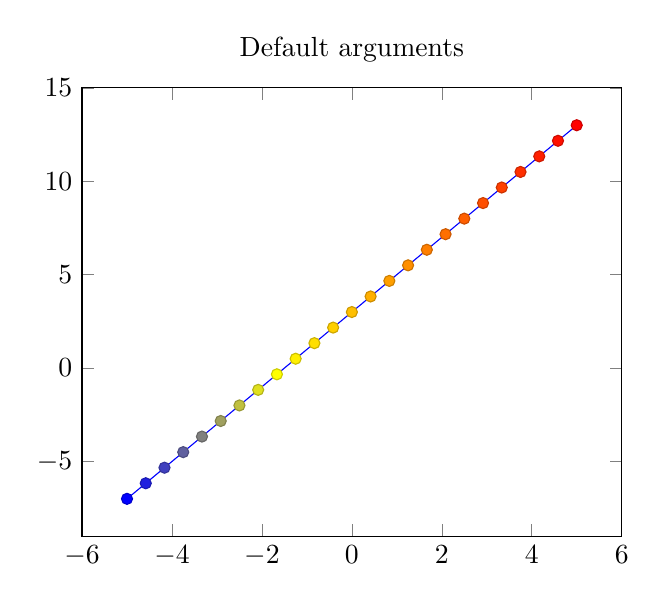
\begin{tikzpicture}
\begin{axis}[title=Default arguments]
\addplot+[scatter,scatter src=y]
	{2*x+3};
\end{axis}
\end{tikzpicture}
\end{codeexample}

\begin{codeexample}[]
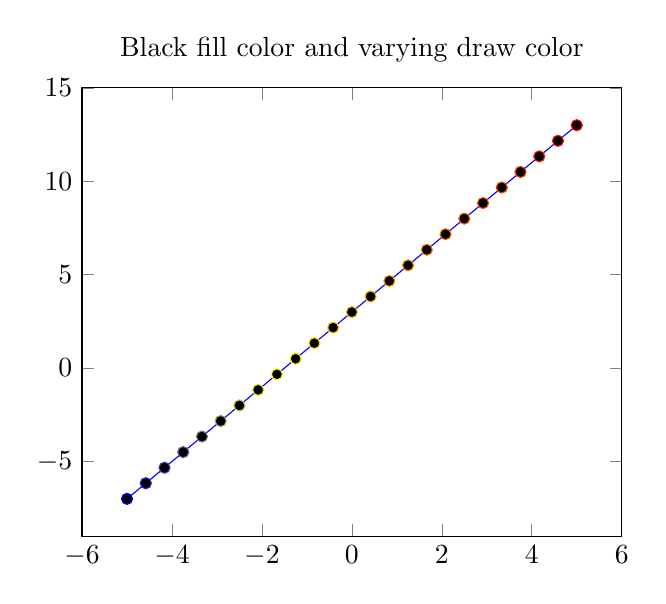
\begin{tikzpicture}
\begin{axis}[
	title=Black fill color and varying draw color,
	scatter/use mapped color=
		{draw=mapped color,fill=black}]
\addplot+[scatter,scatter src=y]
	{2*x+3};
\end{axis}
\end{tikzpicture}
\end{codeexample}

\begin{codeexample}[]
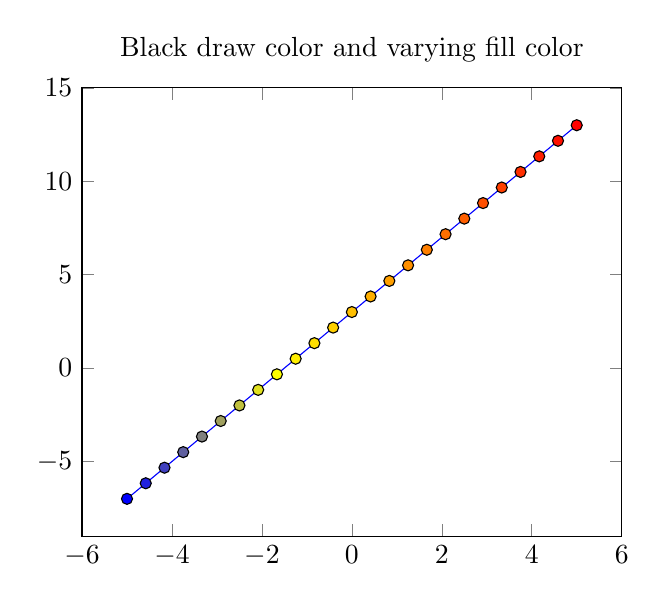
\begin{tikzpicture}
\begin{axis}[
	title=Black draw color and varying fill color,
	scatter/use mapped color=
		{draw=black,fill=mapped color}]
\addplot+[scatter,scatter src=y]
	{2*x+3};
\end{axis}
\end{tikzpicture}
\end{codeexample}
	This key is actually a style which redefines |@pre marker code| and |@post marker code| (see below).

	\paragraph{Remark:} The style |use mapped color| \emph{re}defines |@pre marker code| and |@post marker code|. There is a starred variant \declareandlabel{use mapped color*} which \emph{appends} the functionality while keeping the old marker code.
\end{stylekey}

\begin{stylekey}{/pgfplots/scatter/classes=\marg{styles for each class name}}
\label{pgfplots:scatterclasses}
	A scatter plot style which visualizes points using several classes. The style assumes that every point coordinate has a class label attached, that means the choice |scatter src=explicit symbolic| is assumed\footnote{If \texttt{scatter src} is not \texttt{explicit symbolic}, we expect a numeric argument which is rounded to the nearest integer. The resulting integer is used a class label. If that fails, the numeric argument is truncated to the nearest integer. If that fails as well, the point has no label.}. A class label can be a number, but it can also be a symbolic constant. Given class labels for every point, \marg{styles for each class name} contains a comma-separated list which associates appearance options to each class label.

\begin{codeexample}[]
\begin{tikzpicture}
\begin{axis}[scatter/classes={
	a={mark=square*,blue},%
	b={mark=triangle*,red},%
	c={mark=o,draw=black}}]

	% \addplot[] is better than \addplot+[] here:
	% it avoids scalings of the cycle list
	\addplot[scatter,only marks,
		scatter src=explicit symbolic]
		coordinates {
			(0.1,0.15)  [a]
			(0.45,0.27) [c]
			(0.02,0.17) [a]
			(0.06,0.1)  [a]
			(0.9,0.5)   [b]
			(0.5,0.3)   [c]
			(0.85,0.52) [b]
			(0.12,0.05) [a]
			(0.73,0.45) [b]
			(0.53,0.25) [c]
			(0.76,0.5)  [b]
			(0.55,0.32) [c]
		};
\end{axis}
\end{tikzpicture}
\end{codeexample}
In this example, the coordinate |(0.1,0.15)| has the associated label `|a|' while |(0.45,0.27)| has the label `|c|' (see section~\ref{sec:addplot} for details about specifying point meta data). Now, The argument to |scatter/classes| contains styles for every label -- for label `|a|', square markers will be drawn in color blue. 

The generation of a legend works as for a normal plot -- but |scatter/classes| requires one legend entry for every provided class. It communicates the class labels to the legend automatically. It works as if there had been different |\addplot| commands, one for every class label.

It is also possible to provide |scatter/classes| as argument to a single plot, allowing different scatter plots in one axis.
\begin{codeexample}[]
\begin{tikzpicture}
\begin{axis}[legend pos=south east]
	% The data file contains:
	% x     y      label
	% 0.1   0.15   a 
	% 0.45  0.27   c 
	% 0.02  0.17   a 
	% 0.06  0.1    a 
	% 0.9   0.5    b 
	% 0.5   0.3    c 
	% 0.85  0.52   b 
	% 0.12  0.05   a 
	% 0.73  0.45   b 
	% 0.53  0.25   c 
	% 0.76  0.5    b 
	% 0.55  0.32   c 
    \addplot[
		scatter/classes={
			a={mark=square*,blue},%
			b={mark=triangle*,red},%
			c={mark=o,draw=black,fill=black}%
		},
		scatter,only marks,
		scatter src=explicit symbolic]
	table[x=x,y=y,meta=label]
			{plotdata/scattercl.dat};

	\addplot coordinates 
		{(0.1,0.1) (0.5,0.3) (0.85,0.5)};
	\legend{Class 1,Class 2,Class 3,Line}
\end{axis}
\end{tikzpicture}
\end{codeexample}

In general, the format of \marg{styles for each class name} is a comma separated list of \meta{label}|=|\marg{style options}.

\paragraph{Attention:} The keys |every mark| and |mark options| have \emph{no effect} when used inside of \marg{styles for each class name}! So, instead of assigning |mark options|, you can simply provide the options directly. They apply only to markers anyway.

\paragraph{Remark:} To use |\label| and |\ref| in conjunction with |scatter/classes|, you can provide the class labels as optional arguments to |\label| in square brackets:

\begin{codeexample}[code only]
\addplot[
	scatter/classes={
		a={mark=square*,blue},%
		b={mark=triangle*,red},%
		c={mark=o,draw=black,fill=black}%
	},
	scatter,only marks,
	scatter src=explicit symbolic]
	% [and coordinate input here... ]
	;

\label[a]{label:for:first:class}
\label[b]{label:for:second:class}
\label[c]{label:for:third:class}

...
First class is \ref{label:for:first:class}, second is \ref{label:for:second:class}.
\end{codeexample}

	\paragraph{Remark:} The style |scatter/classes| \emph{re}defines |@pre marker code| and |@post marker code|. There is a starred variant \declareandlabel{scatter/classes*} which \emph{appends} the functionality while keeping the old marker code.
\end{stylekey}

\begin{pgfplotskey}{nodes near coords=\marg{content} (default \textbackslash pgfmathprintnumber\textbackslash pgfplotspointmeta)}
	A |scatter| plot style which places text nodes near every coordinate.

\begin{codeexample}[]
\begin{tikzpicture}
\begin{axis}[nodes near coords]
	\addplot+[only marks] coordinates {
		(0.5,0.2) (0.2,0.1) (0.7,0.6) 
		(0.35,0.4) (0.65,0.1)};
\end{axis}
\end{tikzpicture}
\end{codeexample}
	The \marg{content} is, if nothing else has been specified, the content of the ``point meta'', displayed using the default \meta{content}=|\pgfmathprintnumber{\pgfplotspointmeta}|. The macro |\pgfplotspointmeta| contains whatever has been selected by the |point meta| key, it defaults to the $y$ coordinate for two dimensional plots and the $z$ coordinate for three dimensional plots.

	Since |point meta=explicit symbolic| allows to treat string data, you can provide textual descriptions which will be shown inside of the generated nodes\footnote{In this case, the |\textbackslash pgfmathprintnumber| will be skipped automatically.}:

\begin{codeexample}[]
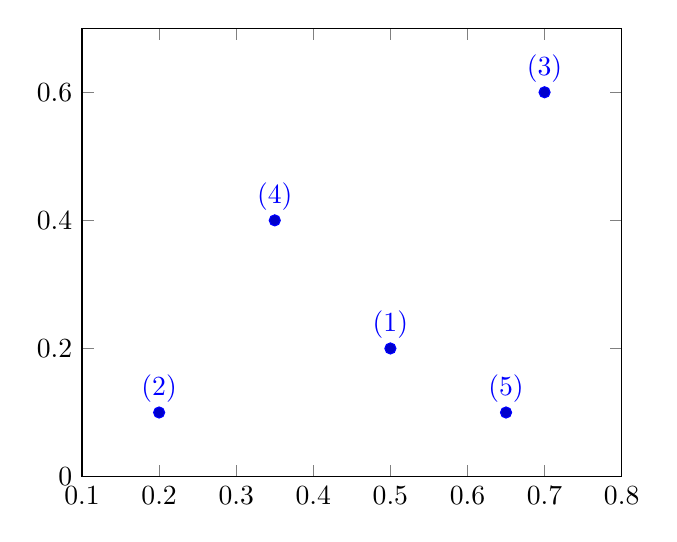
\begin{tikzpicture}
\begin{axis}[nodes near coords,enlargelimits=0.2]
	\addplot+[only marks,
		point meta=explicit symbolic] 
	coordinates {
		(0.5,0.2) [(1)]
		(0.2,0.1) [(2)]
		(0.7,0.6) [(3)]
		(0.35,0.4) [(4)]
		(0.65,0.1) [(5)]
	};
\end{axis}
\end{tikzpicture}
\end{codeexample}
	The square brackets are the way to provide explicit |point meta| for |plot coordinates|. Please refer to the documentation of |plot file| and |plot table| for how to get point meta from files.

	The style |nodes near coords| might be useful for bar plots, see |ybar| for an example of |nodes near coords|.

	\paragraph{Remarks and Details:}
	\begin{itemize}
		\item |nodes near coords| uses the same options for line styles and colors as the current plot. This may be changed using the style |every node near coord|, see below.

		\item |nodes near coords| is actually one of the |scatter| plot styles. It redefines |scatter/@pre marker code| to generate several \Tikz\ |\node| commands.

		In order to use |nodes near coords| together with other |scatter| plot styles (like |scatter/use mapped color| or |scatter/classes|), you may append a star to each of these keys. The variant \declareandlabel{nodes near coords*} will \emph{append} code to |scatter/@pre marker code| without overwriting the previous value.
		\item Consider using |enlargelimits| together with |nodes near coords| if text is clipped away.
		\item Currently |nodes near coords| does not work satisfactory for |ybar interval| or |xbar interval|, sorry.

	\end{itemize}
\end{pgfplotskey}

\begin{stylekey}{/pgfplots/every node near coord}
	A style used for every node generated by |nodes near coords|. It is initially empty.
\end{stylekey}

\begin{pgfplotskey}{nodes near coords align=\marg{alignment method} (initially auto)}
	Specifies how to align nodes generated by |nodes near coords|. 

	Possible choices for \marg{alignment} are

	\begin{description}
		\item[]\declare{auto} Uses |horizontal| if the $x$ coordinates are shown or |vertical| in all other cases. This checks the current value of |point meta|.
		\item[]\declare{horizontal} uses |left| if |\pgfplotspointmeta| $<0$ and |right| otherwise.
		\item[]\declare{vertical}   uses |below| if |\pgfplotspointmeta| $<0$ and |above| otherwise.
		\item[] Its also possible to provide any \Tikz\ alignment option such as |anchor=north east|, |below| or something like that. It is also allowed if multiple options are provided.
	\end{description}
\end{pgfplotskey}


\begin{pgfplotsxycodekeylist}{
	scatter/@pre marker code,
	scatter/@post marker code}
	These two keys constitute the public interface which determines the marker appearance depending on scatter source coordinates.

	Redefining them allows fine grained control even over marker types, line styles and colors.

	The scatter plot algorithm works as follows:
\begin{enumerate} 
\item The scatter source coordinates form a data stream whose data limits are computed additionally to the axis limits. This step is skipped for |symbolic| meta data.
\item Before any markers are drawn, a linear coordinate transformation from these data limits to the interval $[0.0,1000.0]$ is initialised. 
\item Every scatter source coordinate\footnote{During the evaluation, the public macros \texttt{\textbackslash pgfplotspointmeta} and \texttt{\textbackslash pgfplotspointmetarange} indicate the source coordinate and the source coordinate range in the format $a:b$ (for log--axis, they are given in fixed point representation and for linear axes in floating point).} will be transformed linearly and the result is available as macro |\pgfplotspointmetatransformed| $ \in [0.0,1000.0]$.

The decision is thus based on per thousands of the data range. The transformation is skipped for |symbolic| meta data (and the meta data is simply contained in the mentioned macro).
\item The \pgfname\ coordinate system is translated such that |(0pt,0pt)| is the plot coordinate.
\item The code of |scatter/@pre marker code| is evaluated (without arguments).
\item The standard code which draws markers is evaluated.
\item The code of |scatter/@post marker code| is evaluated (without arguments).
\end{enumerate}
	The idea is to generate a set of appearance keys which depends on |\pgfplotspointmetatransformed|. Then, a call to |\scope|\oarg{generated keys} as |@pre| code and the associated |\endscope| as |@post| code will draw markers individually using \oarg{generated keys}.

A technical example is shown below. It demonstrates how to write user defined routines, in this case a three--class system\footnote{Please note that you don't need to copy this particular example: the multiple--class example is also available as predefined style \texttt{scatter/classes}.}.
\begin{codeexample}[]
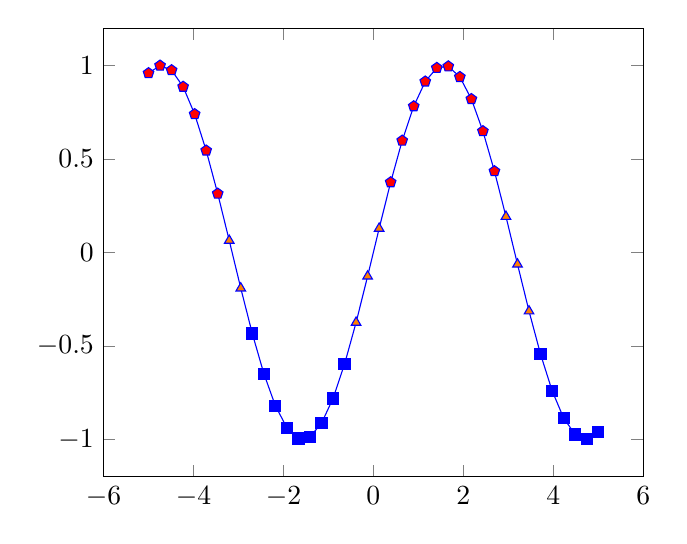
\begin{tikzpicture}
% Low-Level scatter plot interface Example: 
% use three different marker classes 
% 0% - 30%   : first class
% 30% - 60%  : second class
% 60% - 100% : third class
\begin{axis}[
scatter/@pre marker code/.code={%
   \ifdim\pgfplotspointmetatransformed pt<300pt
      \def\markopts{mark=square*,fill=blue}%
   \else
      \ifdim\pgfplotspointmetatransformed pt<600pt
         \def\markopts{mark=triangle*,fill=orange}%
      \else
         \def\markopts{mark=pentagon*,fill=red}%
      \fi
   \fi
   \expandafter\scope\expandafter[\markopts]
},%
scatter/@post marker code/.code={%
   \endscope
}]

\addplot+[scatter,scatter src=y,
	samples=40]
   {sin(deg(x))};
   
\end{axis}
\end{tikzpicture}
\end{codeexample}
Please note that |\ifdim| compares \TeX\ lengths, so the example employs the suffix |pt| for any number used in this context. That doesn't change the semantics. The two (!) |\expandafter| constructions make sure that |\scope| is invoked with the \emph{content} of |\markopts| instead of the macro name |\markopts|.
\end{pgfplotsxycodekeylist}

\subsubsection{1D Colored Mesh Plots}
\begin{plottype}[/pgfplots]{mesh}
	Uses the current color map to determine colors for each fixed line segment. Each line segment will get the same color.
\begin{codeexample}[]
\begin{tikzpicture}
	\begin{axis}
	\addplot[mesh] {x+sin(deg(x))};
	\end{axis}
\end{tikzpicture}
\end{codeexample}
	The color data is per default the $y$ value of the plot. It can be reconfigured using the |point meta| key (which is actually the same as |scatter src|). The following example provides the color data explicitly for |plot coordinates|, using the square bracket notation.
\begin{codeexample}[]
\begin{tikzpicture}
	\begin{axis}
	\addplot[mesh,point meta=explicit] 
		coordinates {
			(0,0)   [0]
			(1,0.1) [1]
			(2,0.1) [2]
			(3,0.3) [3]
			(4,0.3) [4]
		};
	\end{axis}
\end{tikzpicture}
\end{codeexample}
	This onedimensional |mesh| plot is actually a special case of the twodimensional mesh plots, so more detailed configuration, including how to change the color data, can be found in section~\ref{sec:2d:mesh}.

\end{plottype}


\subsubsection{Interrupted Plots}
\index{Interrupted Plots}%
\label{pgfplots:interrupt}%
Sometimes it is desirable to draw parts of a single plot separately, without connection between the parts (discontinuities). This can be achieved using the |unbounded coords| key combined with coordinate values |nan|, |inf| or |-inf|.

\begin{pgfplotskey}{unbounded coords=\mchoice{discard,jump} (initially discard)}
	This key configures what to do if one or more coordinates of a single point are unbounded. Here, unbounded means it is either $\pm \infty$ (|+inf| or |-inf|) or it has the special ``not--a--number'' value |nan|.

	The initial setting \declaretext{discard} discards the complete point and a warning is issued in the log file\footnote{The warning can be disabled with \texttt{filter discard warning=false}.}. This setting has the same effect as if the unbounded point did not occur: \PGFPlots\ will interpolate between the bounded adjacent points.

	The alternative \declaretext{jump} allows interrupted plots: it provides extra checking for these coordinates and does not interpolate over them; only those line segments which are adjacent to unbounded coordinates will be skipped. 
\begin{codeexample}[]
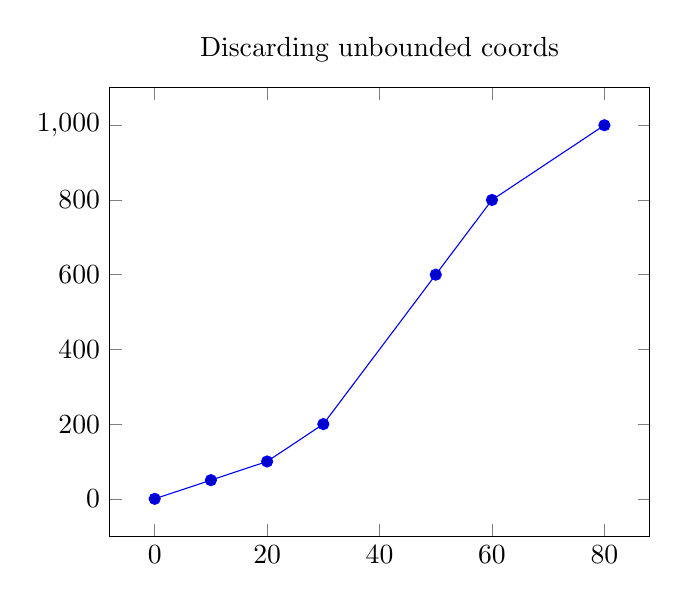
\begin{tikzpicture}
\begin{axis}[
	title=Discarding unbounded coords,
	unbounded coords=discard]

	\addplot coordinates {
		(0,0) (10,50) (20,100) (30,200) 
		(40,inf) (50,600) (60,800) (80,1000)
	};
\end{axis}
\end{tikzpicture}
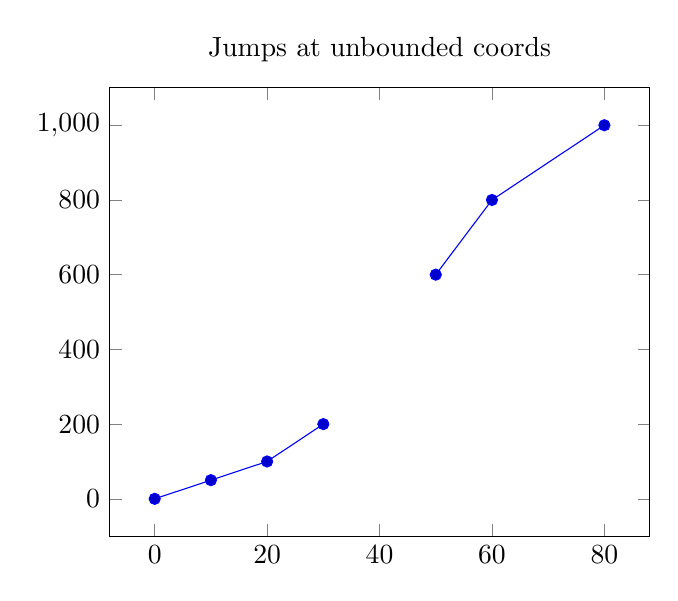
\begin{tikzpicture}
\begin{axis}[
	title=Jumps at unbounded coords,
	unbounded coords=jump]
	\addplot coordinates {
		(0,0) (10,50) (20,100) (30,200) 
		(40,inf) (50,600) (60,800) (80,1000)
	};
\end{axis}
\end{tikzpicture}
\end{codeexample}

	For plot expression and its friends, it is more likely to get very large floating point numbers instead of |inf|. In this case, consider using the |restrict x to domain| key described on page~\pageref{key:restrict:x:to:domain}.

	The |unbounded coords=jump| method does also work for mesh/surface plots: every face adjacent to an unbounded coordinate will be discarded in this case. The following example sets up a (cryptic) coordinate filter which cuts out a quarter of the domain and replaces its values with |nan|:

\pgfplotsexpensiveexample
\begin{codeexample}[]
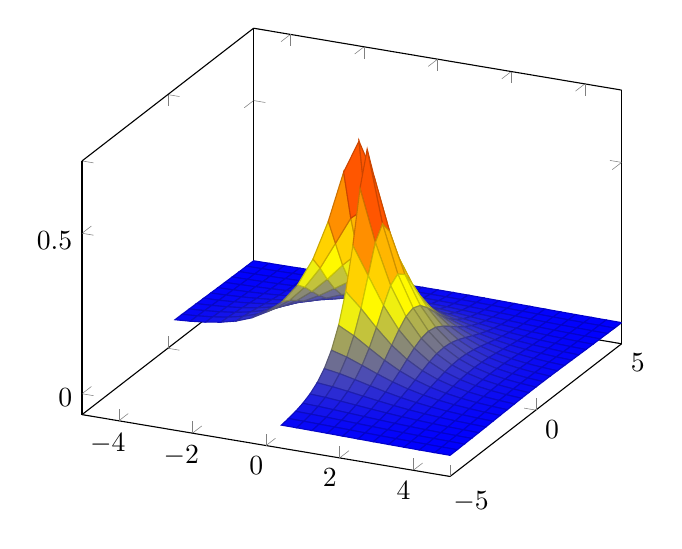
\begin{tikzpicture}
\begin{axis}[
  unbounded coords=jump,
  % A technical filter to cut out 
  % the x<0 and y<0 edge.
  filter point/.code={%
    \pgfmathparse
      {\pgfkeysvalueof{/data point/x}<0}%
    \ifpgfmathfloatcomparison
      \pgfmathparse
        {\pgfkeysvalueof{/data point/y}<0}%
      \ifpgfmathfloatcomparison
        \pgfkeyssetvalue{/data point/x}{nan}%
      \fi
    \fi
  },
  ]
  \addplot3[surf] {exp(-sqrt(x^2 + y^2))};
\end{axis}
\end{tikzpicture}
\end{codeexample}
\end{pgfplotskey}

